\documentclass{beamer}
\usetheme{CambridgeUS}
\usepackage[french]{babel}
\usepackage{fontspec}
\usepackage{graphicx}
\usepackage{textcomp}
\usepackage{import}
\usepackage{tabu}
\usepackage{makecell}
\usepackage{colortbl}
\usepackage{arydshln}
\usepackage{multirow}
\usepackage{pgffor}

\usepackage{minted}
\usemintedstyle{trac}
\newmintedfile[python]{python}{
    tabsize=4,
    linenos,
    frame=lines,
    framesep=2mm
}
\renewcommand\theFancyVerbLine{\arabic{FancyVerbLine}}

% More vertical spacing in tabu lines
\tabulinesep=1.5mm

\graphicspath{{figures/}}
\useinnertheme{rectangles}
\setbeamertemplate{blocks}[default]

\title[Environnement pour l'exploration visuelle]{Environnement logiciel pour l'apprentissage de l'exploration visuelle d'une image}
\author{Louis Cuni \and Pablo Donato}
\institute[]{Université Pierre et Marie Curie -- Paris VI}
\date{2 mai 2017}
\subject{3I013 -- Introduction à la recherche}

%\setcounter{tocdepth}{1}
%\AtBeginSection[]
%{
    %\begin{frame}
        %\frametitle{Sommaire}
        %\tableofcontents[currentsection]
    %\end{frame}
%}

\begin{document}

\frame{\titlepage}

\begin{frame}
    \frametitle{Sommaire}
    \tableofcontents
\end{frame}

\section{Introduction}

\begin{frame}
    \frametitle{Contexte}
    \begin{columns}[T]
        \begin{column}{.48\textwidth}
            \center
            \begin{block}{Environnement}
                TODO
            \end{block}
            \begin{block}{Agent}
                TODO
            \end{block}
        \end{column}
        \begin{column}{.48\textwidth}
            \begin{figure}
                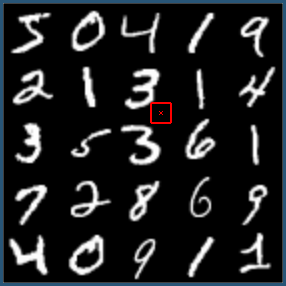
\includegraphics[height=0.5\textheight]{numgrid.png}
            \end{figure}
        \end{column}
    \end{columns}
\end{frame}

\begin{frame}
    \frametitle{Interaction agent-environnement}
    \center
    \begin{figure}
        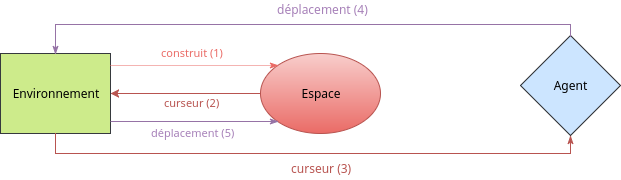
\includegraphics[width=0.9\textwidth]{agent_env_loop.png}
    \end{figure}
    \vspace{3em}
    \begin{enumerate}
        \item Construction de l'\textbf{espace}
        \item Boucle d'interaction
    \end{enumerate}
\end{frame}

\section{Environnement}

\begin{frame}
    \frametitle{Chargement de la grille}
    \begin{columns}[c]
        \begin{column}{.48\textwidth}
            \begin{block}{MNIST}
                \begin{itemize}
                    \item images + labels
                    \item training set + testing set
                \end{itemize}
            \end{block}
            \uncover<2->{
            \begin{block}{Sous-ensemble de chiffres}
                \begin{enumerate}
                    \item Chargement des labels
                    \item Sélection des indices
                    \item Chargement des images
                    \item Sélection des labels
                \end{enumerate}
            \end{block}}
        \end{column}
        \uncover<2->{
        \begin{column}{.48\textwidth}
            \center
            \fontsize{4pt}{7}\selectfont
            \python{code/loadgrid.py}
        \end{column}}
    \end{columns}
\end{frame}

\begin{frame}
    \frametitle{Apprentissage par renforcement}
    \begin{columns}[c]
        \begin{column}{.44\textwidth}
            \begin{block}{IA}
                \begin{itemize}
                    \item Classe d'algorithmes d'apprentissage
                    \item Inspiré de la psychologie animale
                \end{itemize}
            \end{block}
            \uncover<2->{
            \begin{block}{Cadre formel : \textsc{mdp}}
                \begin{enumerate}
                    \item Ensemble d'états $S$
                    \item Ensemble d'actions $A$
                    \item Ensemble de récompenses $R$
                    \item Fonction de probabilités $p$
                \end{enumerate}
            \end{block}}
        \end{column}
        \uncover<2->{
        \begin{column}{.52\textwidth}
            \center
            \fontsize{5.5pt}{7}\selectfont
            \begin{tabu}{|c|c|c|}\hline
                Espace & Attribut & Classe \\ \hline
                $D = \{0,1,\ldots,10\}$ & \texttt{digit\_space} & \texttt{Discrete} \\ \hline
                $P = P_x \times P_y$ & \texttt{position\_space} & \texttt{MultiDiscrete} \\ \hline
                $A = P \times D$ & \texttt{action\_space} & \texttt{Tuple} \\ \hline
                $S = [0;255]^{h \times w}$ & \texttt{observation\_space} & \texttt{Box} \\ \hline
            \end{tabu}
        \end{column}}
    \end{columns}
\end{frame}

\begin{frame}
    \frametitle{Espaces et wrappers}
    \fontsize{9pt}{7}\selectfont
    \begin{block}{Wrapper}
        \begin{itemize}
            \item $\Leftrightarrow$ Design pattern \textit{décorateur} pour \texttt{gym.Env}
            \item Conversion espaces d'actions/états (\texttt{ActionWrapper}/\texttt{ObservationWrapper})
        \end{itemize}
    \end{block}
    \uncover<2->{
    \begin{block}{Pour \texttt{NumGrid}}
        \begin{itemize}
            \item \texttt{DirectionWrapper}
            \item \texttt{DiscreteDirectionWrapper}
            \item \texttt{DiscretePositionWrapper}
            \item \texttt{DiscreteActionWrapper}
        \end{itemize}
    \end{block}
    \center
    \fontsize{8pt}{7}\selectfont
    \python{code/wrappers.py}}
\end{frame}

\begin{frame}
    \frametitle{Méthode \texttt{step}}
    \fontsize{9pt}{7}\selectfont
    \begin{columns}[c]
        \begin{column}{.53\textwidth}
            \begin{block}{Fonction}
                \begin{itemize}
                    \item 1 pas de temps boucle d'interaction
                    \item Fournit les informations à l'agent
                \end{itemize}
            \end{block}
            \uncover<2->{
            \begin{block}{Opérations}
                \begin{enumerate}
                    \item Vérification position curseur
                    \item Déplacement curseur
                    \item Choix récompense
                    \item Changement de zone
                    \item Vérification fin épisode
                    \item Retour des informations
                \end{enumerate}
            \end{block}}
        \end{column}
        \uncover<2->{
        \begin{column}{.43\textwidth}
            \center
            \fontsize{4.5pt}{7}\selectfont
            \python{code/step.py}
        \end{column}}
    \end{columns}
\end{frame}

\section{Agent}

\begin{frame}
    \frametitle{Réseaux de neurones}
    \begin{columns}[T]
        \begin{column}{.48\textwidth}
            \begin{figure}
                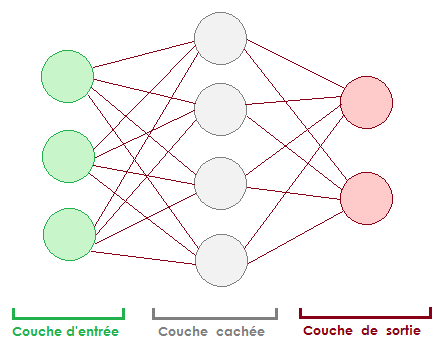
\includegraphics[width=\textwidth]{neuralnet.png}
            \end{figure}
        \end{column}
        \begin{column}{.48\textwidth}
            \begin{figure}
                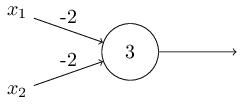
\includegraphics[width=0.8\textwidth]{neuron.png}
            \end{figure}
            \begin{block}{}
                \center
                Commentaires ?
            \end{block}
        \end{column}
    \end{columns}
\end{frame}

\begin{frame}
    \frametitle{Prédicteurs}
    \begin{figure}
        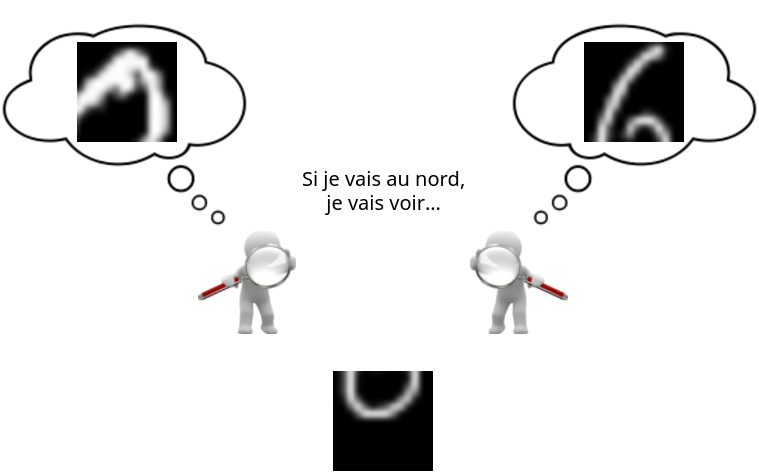
\includegraphics[width=0.9\textwidth]{slide_predicter.png}
    \end{figure}
\end{frame}

\newcommand{\predicterguy}[1]{
    \begin{minipage}{.15\textwidth}
        \center
        \includegraphics[width=0.75\linewidth]{predicter_guy_#1.png}
    \end{minipage}}

\newcommand{\pls}{\cellcolor{blue!20}}
\newcommand{\win}{\cellcolor{green!20}}

\begin{frame}[t]
    \frametitle{Prise de décisions}
    \fontsize{7pt}{7}\selectfont
    \center

    \only<1>{
    \begin{tabu}{|c|c|c|c|} \hline
        \predicterguy{1} & \predicterguy{2} & \predicterguy{3} & $t$ \\ \hline
    \end{tabu}}

    \only<2>{
    \begin{tabu}{|c|c|c|c|} \hline
        \predicterguy{1} & \predicterguy{2} & \predicterguy{3} & $t$ \\ \hline
        0 & 0 & 0 & \multirow{2}{*}{0} \\ \cdashline{1-3}[1pt/1.5pt]
        0 & 0 & 0 & \\ \hline
    \end{tabu}}

    \only<3>{
    \begin{tabu}{|c|c|c|c|} \hline
        \predicterguy{1} & \predicterguy{2} & \predicterguy{3} & $t$ \\ \hline
        0 & 0 & 0 & \multirow{2}{*}{0} \\ \cdashline{1-3}[1pt/1.5pt]
        0 & 0 & 0 & \\ \hline
        0.81 & 0.86 & 0.83 & \multirow{2}{*}{1} \\ \cdashline{1-3}[1pt/1.5pt]
        0 & 0 & 0 & \\ \hline
    \end{tabu}}

    \only<4>{
    \begin{tabu}{|c|c|c|c|} \hline
        \predicterguy{1} & \predicterguy{2} & \predicterguy{3} & $t$ \\ \hline
        0 & 0 & 0 & \multirow{2}{*}{0} \\ \cdashline{1-3}[1pt/1.5pt]
        0 & 0 & 0 & \\ \hline
        0.81 & 0.86 \pls & 0.83 & \multirow{2}{*}{1} \\ \cdashline{1-3}[1pt/1.5pt]
        0 & 1 & 0 & \\ \hline
    \end{tabu}}

    \only<5>{
    \begin{tabu}{|c|c|c|c|} \hline
        \predicterguy{1} & \predicterguy{2} & \predicterguy{3} & $t$ \\ \hline
        0 & 0 & 0 & \multirow{2}{*}{0} \\ \cdashline{1-3}[1pt/1.5pt]
        0 & 0 & 0 & \\ \hline
        0.81 & 0.86 \pls & 0.83 & \multirow{2}{*}{1} \\ \cdashline{1-3}[1pt/1.5pt]
        0 & 1 & 0 & \\ \hline
        0.84 & 0.83 & 0.80 & \multirow{2}{*}{2} \\ \cdashline{1-3}[1pt/1.5pt]
        0 & 1 & 0 & \\ \hline
    \end{tabu}}

    \only<6>{
    \begin{tabu}{|c|c|c|c|} \hline
        \predicterguy{1} & \predicterguy{2} & \predicterguy{3} & $t$ \\ \hline
        0 & 0 & 0 & \multirow{2}{*}{0} \\ \cdashline{1-3}[1pt/1.5pt]
        0 & 0 & 0 & \\ \hline
        0.81 & 0.86 \pls & 0.83 & \multirow{2}{*}{1} \\ \cdashline{1-3}[1pt/1.5pt]
        0 & 1 & 0 & \\ \hline
        0.84 \pls & 0.83 & 0.80 & \multirow{2}{*}{2} \\ \cdashline{1-3}[1pt/1.5pt]
        1 & 1 & 0 & \\ \hline
    \end{tabu}}

    \only<7>{
    \begin{tabu}{|c|c|c|c|} \hline
        \predicterguy{1} & \predicterguy{2} & \predicterguy{3} & $t$ \\ \hline
        0 & 0 & 0 & \multirow{2}{*}{0} \\ \cdashline{1-3}[1pt/1.5pt]
        0 & 0 & 0 & \\ \hline
        0.81 & 0.86 \pls & 0.83 & \multirow{2}{*}{1} \\ \cdashline{1-3}[1pt/1.5pt]
        0 & 1 & 0 & \\ \hline
        0.84 \pls & 0.83 & 0.80 & \multirow{2}{*}{2} \\ \cdashline{1-3}[1pt/1.5pt]
        1 & 1 & 0 & \\ \hline
        0.82 & 0.89 & 0.85 & \multirow{2}{*}{3} \\ \cdashline{1-3}[1pt/1.5pt]
        1 & 1 & 0 & \\ \hline
    \end{tabu}}

    \only<8>{
    \begin{tabu}{|c|c|c|c|} \hline
        \predicterguy{1} & \predicterguy{2} & \predicterguy{3} & $t$ \\ \hline
        0 & 0 & 0 & \multirow{2}{*}{0} \\ \cdashline{1-3}[1pt/1.5pt]
        0 & 0 & 0 & \\ \hline
        0.81 & 0.86 \pls & 0.83 & \multirow{2}{*}{1} \\ \cdashline{1-3}[1pt/1.5pt]
        0 & 1 & 0 & \\ \hline
        0.84 \pls & 0.83 & 0.80 & \multirow{2}{*}{2} \\ \cdashline{1-3}[1pt/1.5pt]
        1 & 1 & 0 & \\ \hline
        0.82 & 0.89 \pls & 0.85 & \multirow{2}{*}{3} \\ \cdashline{1-3}[1pt/1.5pt]
        1 & 2 & 0 & \\ \hline
    \end{tabu}}

    \only<9>{
    \begin{tabu}{|c|c|c|c|} \hline
        \predicterguy{1} & \predicterguy{2} & \predicterguy{3} & $t$ \\ \hline
        0 & 0 & 0 & \multirow{2}{*}{0} \\ \cdashline{1-3}[1pt/1.5pt]
        0 & 0 & 0 & \\ \hline
        0.81 & 0.86 \pls & 0.83 & \multirow{2}{*}{1} \\ \cdashline{1-3}[1pt/1.5pt]
        0 & 1 & 0 & \\ \hline
        0.84 \pls & 0.83 & 0.80 & \multirow{2}{*}{2} \\ \cdashline{1-3}[1pt/1.5pt]
        1 & 1 & 0 & \\ \hline
        0.82 & 0.89 \pls & 0.85 & \multirow{2}{*}{3} \\ \cdashline{1-3}[1pt/1.5pt]
        1 & 2 & 0 & \\ \hline
        0.83 & 0.91 & 0.86 & \multirow{2}{*}{4} \\ \cdashline{1-3}[1pt/1.5pt]
        1 & 2 & 0 & \\ \hline
    \end{tabu}}

    \only<10>{
    \begin{tabu}{|c|c|c|c|} \hline
        \predicterguy{1} & \predicterguy{2} & \predicterguy{3} & $t$ \\ \hline
        0 & 0 & 0 & \multirow{2}{*}{0} \\ \cdashline{1-3}[1pt/1.5pt]
        0 & 0 & 0 & \\ \hline
        0.81 & 0.86 \pls & 0.83 & \multirow{2}{*}{1} \\ \cdashline{1-3}[1pt/1.5pt]
        0 & 1 & 0 & \\ \hline
        0.84 \pls & 0.83 & 0.80 & \multirow{2}{*}{2} \\ \cdashline{1-3}[1pt/1.5pt]
        1 & 1 & 0 & \\ \hline
        0.82 & 0.89 \pls & 0.85 & \multirow{2}{*}{3} \\ \cdashline{1-3}[1pt/1.5pt]
        1 & 2 & 0 & \\ \hline
        0.83 & 0.91 \win & 0.86 & \multirow{2}{*}{4} \\ \cdashline{1-3}[1pt/1.5pt]
        1 & 3 & 0 & \\ \hline
    \end{tabu}}
\end{frame}


\begin{frame}
    \frametitle{Exemple d'une séquence d'identification}
    \center
    \foreach \n in {0,...,11}{
        \only<\n>{
        \begin{figure}
            \includegraphics[height=0.75\textheight]{ident_seq/ident_seq_\n.png}
        \end{figure}}}
\end{frame}

\section{Étude expérimentale}

\begin{frame}
    \frametitle{Architecture des prédicteurs}
    \begin{figure}
        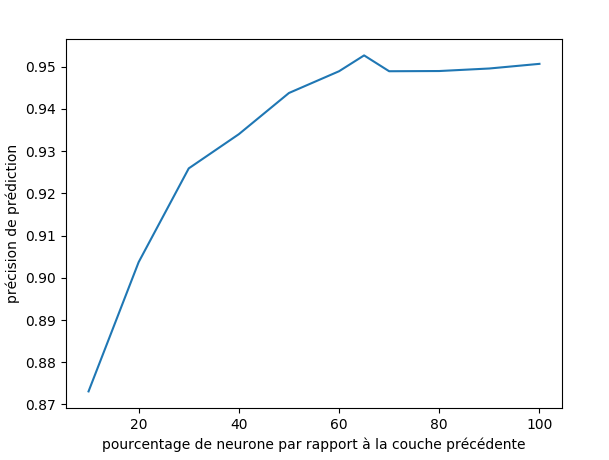
\includegraphics[height=0.5\textheight]{arch_acc.png}
    \end{figure}
    \center
    \fontsize{7pt}{7}\selectfont
    \begin{tabu}{|c|c|c|c|}\hline
        Taille du curseur & Chiffre & Directions & Distance de déplacement \\ \hline
        $8 \times 8$ & 0 & $\{\downarrow\}$ & 1 pixel \\ \hline
    \end{tabu}
\end{frame}

\begin{frame}
    \frametitle{Distance de déplacement}
    \begin{columns}[c]
        \begin{column}{.5\textwidth}
            \begin{figure}
                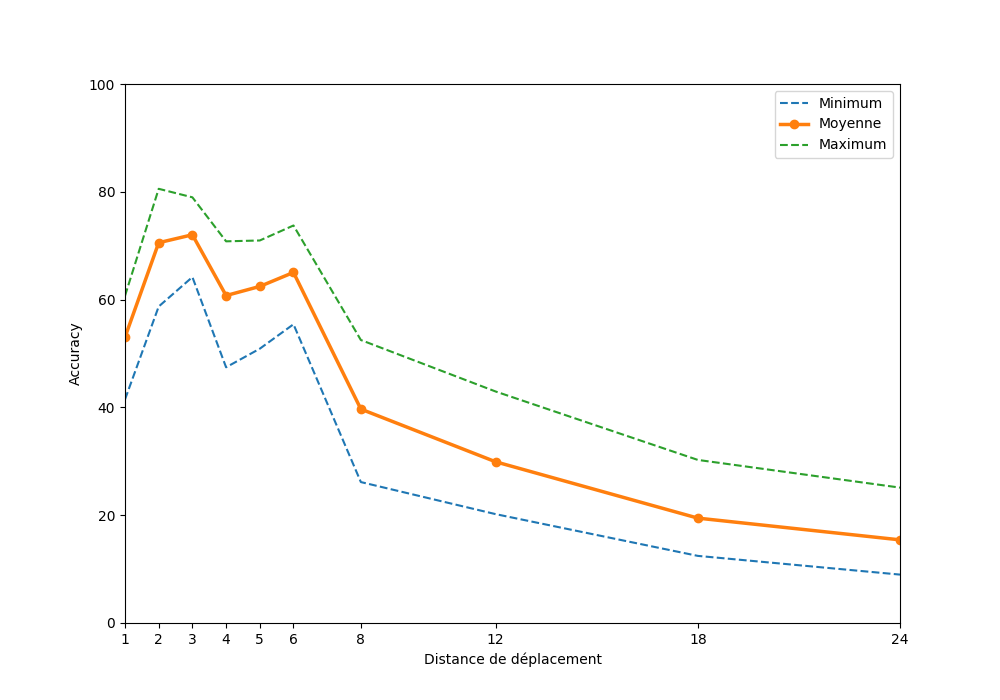
\includegraphics[height=0.5\textheight]{movedist_acc_mean.png}
            \end{figure}
        \end{column}
        \begin{column}{.5\textwidth}
            \begin{figure}
                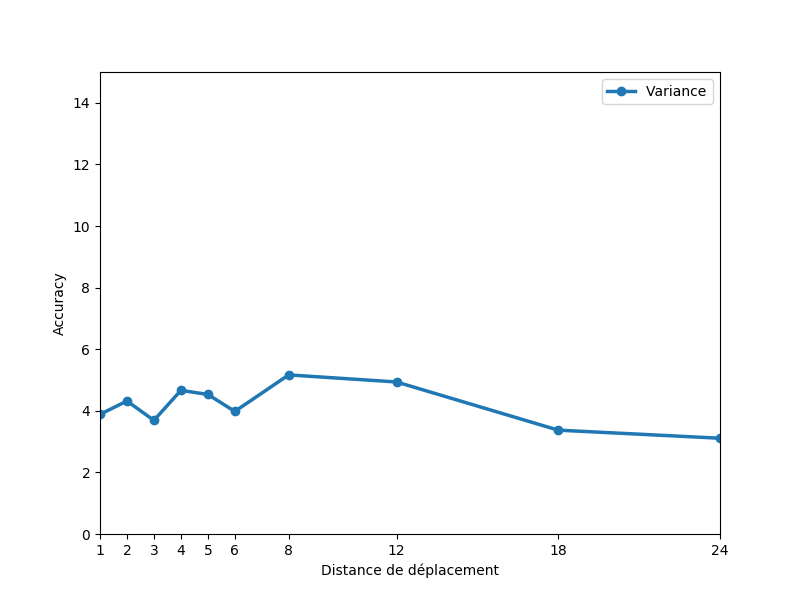
\includegraphics[height=0.45\textheight]{movedist_acc_std.png}
            \end{figure}
        \end{column}
    \end{columns}
    \center
    \fontsize{7pt}{7}\selectfont
    \begin{tabu}{|c|c|c|c|c|}\hline
        Taille de la grille & Chiffres & Taille du curseur & Directions & Seuil de décision \\ \hline
        $1 \times 50$ & Tous & $27 \times 8$ & $\{\downarrow\}$ & 5 \\ \hline
    \end{tabu}
    \vspace{6em}
\end{frame}

\section{Conclusion}

\begin{frame}
    \frametitle{Conclusion}
\end{frame}

\end{document}
